%
% PLAN:
% - ta med "propagating of kappa". At metoden brukt er antagelig ikkje den mest effektive, men det gjøres likt for å lage det meir egna for sammenligning.(ligger i implementation.tex)
% - ta med "om oppsamling av kappa" (ligger i implementation.tex)

%*********************** KANN ***************************
\chapter{implementasjon: KANN}
	Skriv først innledning, med mål om å sette meg og leser på samme utgangsnivå.

	
	\section{Updating $\kappa$} %Calculation and recalculation of $\kappa$
		\subsection{Synaptic transmission}
			% skrive om korleis synaptic transmission fåregår (generellt (om at $\kappa_{ij} = \frac{W_{ij}}{p_{pre}}$ ).
			In biology, a synaptic transmission happens every time a presynaptic action potential is fired.
			The size of this transmission is given by the synaptic weight of the synapse.

			Over some time interval, the total transmisson in a synapse ,$o(\Delta t)$, can be modelled as the synaptic weight times the presynaptic neurons firing frequency times the evaluated time interval.
			We write the presynaptic firing frequency as $f_{pre} = \frac{1}{p_{pre}} = \frac{1}{p(\kappa_{pre})}$ and get:
			\begin{equation}
				\label{eqSynapticTransmission}
				o(\Delta t) = \frac{ W_{ij} }{ p(\kappa_{pre})} * \Delta t 
			\end{equation}

			In discrete--time systems, we can define every synaptic transmission to last for one time iteration (if the time step is large enough).  % MED ELLER IKKJE: "(if the time step is large enough)" ??? XXX
			This causes $\Delta t$ to become constant. We can incoorporate this constant into $W_{ij}$.

			For an ANN based on the activity variable $\kappa$, as previously introduced in chapter \ref{secMatematiskModelleringAvBioNeuron} %TODO Sjekk denne  referansen bedre / skriv bedre (?).
			eq. \eqref{eqSynapticTransmission} is highly relevant.  % highly relevant skurrer litt. Det er veldig relevant. Finn synonym..
			If we define $\Delta t$ to be some constant, and incoorporate this constant into $W_{ij}$, we get the equation for the synaptic transmission of the activity variable.
			We call the size of this transmission $\kappa_{ij}$.

			\begin{equation}
				\label{eqSynapticTransmissionForKANN}
				\kappa_{ij} = \frac{ W_{ij} }{ p(\kappa_{pre})}
			\end{equation}

			For nodes with multiple input synapses, the activity variable $\kappa$ is the sum of all the contributions from different synapses. %VERIFISER DETTE! Vær heilt heilt sikker på at K=sum(K_ij)
			We can write this mathematically as 
			\begin{equation}
				\label{eqSumOfKij}
				\kappa_i = \sum_j{\kappa_{ij}}
			\end{equation}

			In this way the synaptic transmission of the individual synapses can be decoupled from the postsynaptic activity variable, $\kappa_i$.
			
		\subsection{Synaptic input to a node}
			\label{ssecSynInputToANode}
			In $\kappa$ANN we call the nodes for a K\_auron.
			The synaptic input for the activity variable of a K\_auron is defined by \eqref{eqSumOfKij}.
			%To avoid having to recalculate $\kappa_i$ from \eqref{eqSumOfKij} every time the transmission of a synapse changes, we can implement synaptic transmission as the transmission of the derived of $\kappa_{ij}$.
			To avoid recalculation of $\kappa_i$ from all the input synapses when one synapse changes its transmission, this implementation defines edge transmission as the derived of $\kappa_{ij}$.
			Now the postsynaptic $\kappa_i$ can be calculated without summing all the synapse inputs after changed input at one of its edges.
			%In this case the postsynaptic $\kappa$ can be recalucated without summing all the synaptic inputs every time one synapse changes its transmission.

			For synapses transmitting the derived of $\kappa_{ij}$ we only have to integrate this change of transmission from all the input synapses with a changed level of transmission, and get
			\begin{equation}
				\kappa_i = \sum_k{\kappa_{ik}}
			\end{equation}
			Where ${k}$ is a subset of ${j}$ consisting of all the synapses with a changed level of transmission.
			%In the case of only one synapse changing its transmission

			We can, in other words add the change in synaptic transmission, $\Delta K_{ij}$, to the postsynaptic activity variable to get the updated activity variable, $\kappa_i$.
			This can be done at the time of each transmission, and without having to consider any of the other synaptic transmissions to the node.
			
			%XX Skal eg skrive dette her:
			%If we wait until after the current time iteration before calculating the effects of the changed kappa, much calculations will be saved.

			\subsubsection{Effects of the new $\kappa$}
			When $\kappa_i$ changes for a node, we need to recalculate the inverse of the period for this new $\kappa_i$ to get the synaptic transmissions right.
			Because the time step of one time iteration is defined as the smallest time interval in the simulated system, we can define that the propagation of $\kappa$ will happen at the end of the current time iteration. %after this time interval.
			%eller "not instantly".
			Now %If we introduce this as a rule,
			 we can wait until after the current time iteration before calculating the effects of the changed $\kappa_i$.
			%The period of the node, and thus the synaptic transmission of its synapses can in this case wait to after the current time iteration before calculating the effect of the new $\kappa_i$.
			This includes recalculating the estimated firing time, the period inverse and thus the synaptic transmission, and initiate the new time window by calculating the initial depolarization of the neuron and setting 
				ulStartOfTimeWindow for the next time window.

			If we wait til after the current time iteration before calculating the effect of the changed kappa, the above calculations can be done once per time iteration instead of once for each input to the node.
																													% Og vil auke effektiviteten stort!
			This can be wieved as a time delay in the neuron, and is probably  very short compared to what it should be. % TODO: Skriv i Discussion: 
															%At denne delayen er antaklig alt for liten. Dersom eg hadde tid ville eg utforska kor lang denne delayen burde være.
															% Veldig vanskelig å vita kva den SKAL være...


			To wait with the recalculation of the variabled affected by the change in $\kappa$, is implemented with the concept of pCalculateTaskQue, introduced in section \ref{secCalcultaionTaskQue}.
			When a nodes $\kappa$ changes value, a pointer to the node is inserted into a specialized que for this use, pCalculateTaskQue.
\begin{lstlisting}
static std::list<timeInterface*> pCalculateTaskQue;
\end{lstlisting}
			This list is static in the time\_class, that is only one variable is made for time\_class (not one per object).
			When time\_class::doTask() runs, it first calls time\_class::doCalculations().
			%First it makes shure that each entry of the list pCalculateTaskQue is unique (it removes any duplicate). 

			The first task of time\_class::doCalculation() is to enshure that each element of pCalculateTaskQue is unique. 
			This is done by iterating through the list and removing all duplicates of each entry.
			
			The next task is to call each of the remaining elements' .doCalculation() function.
			The function doCalculation() is defined as a pure virtual function in timeInterface, and every class that does not define its own doCalculation() remains an interface class.
			This makes shure that every object of a timeInterface derived class have defined a doCalculation() function. This function is defined in the class if to make it possible to make an istance of the class.
			% gitt av kva elementet har behov for å vente med å kalkulere. For K_auron er det effekten av endring av Kappa som er hensiktsmessig å vente med. For s_auron er det kanskje lekkasjen?

			For K\_aurons, the inherited virtual function .doCalculation() has the task of calculating every variable that changes as a consequence of a changed activity variable for the auron.
			% TODO Skriv bedre XXX

			\subsection{Analysis of synaptic transmission as the derived}
			When synaptic transmission is defined as the derived of $\kappa_{ij}$ the gain in efficiency can be noticable. 
			It also introduces some effects that is important to consider. 

			The most imminent effect is the possibility of an integral error from integrating the derived to get the new $\kappa_i$. 
			This is important, and a whole section is dedicated consideration of this (se sec. \ref{ssecRecalcKappa}).



\begin{figure}[hb!tp]
	\centering
	%
   	\subfloat[Presynaptic activity variable, {$\kappa_j$}]{\label{figSynTransmission:edge-a} 						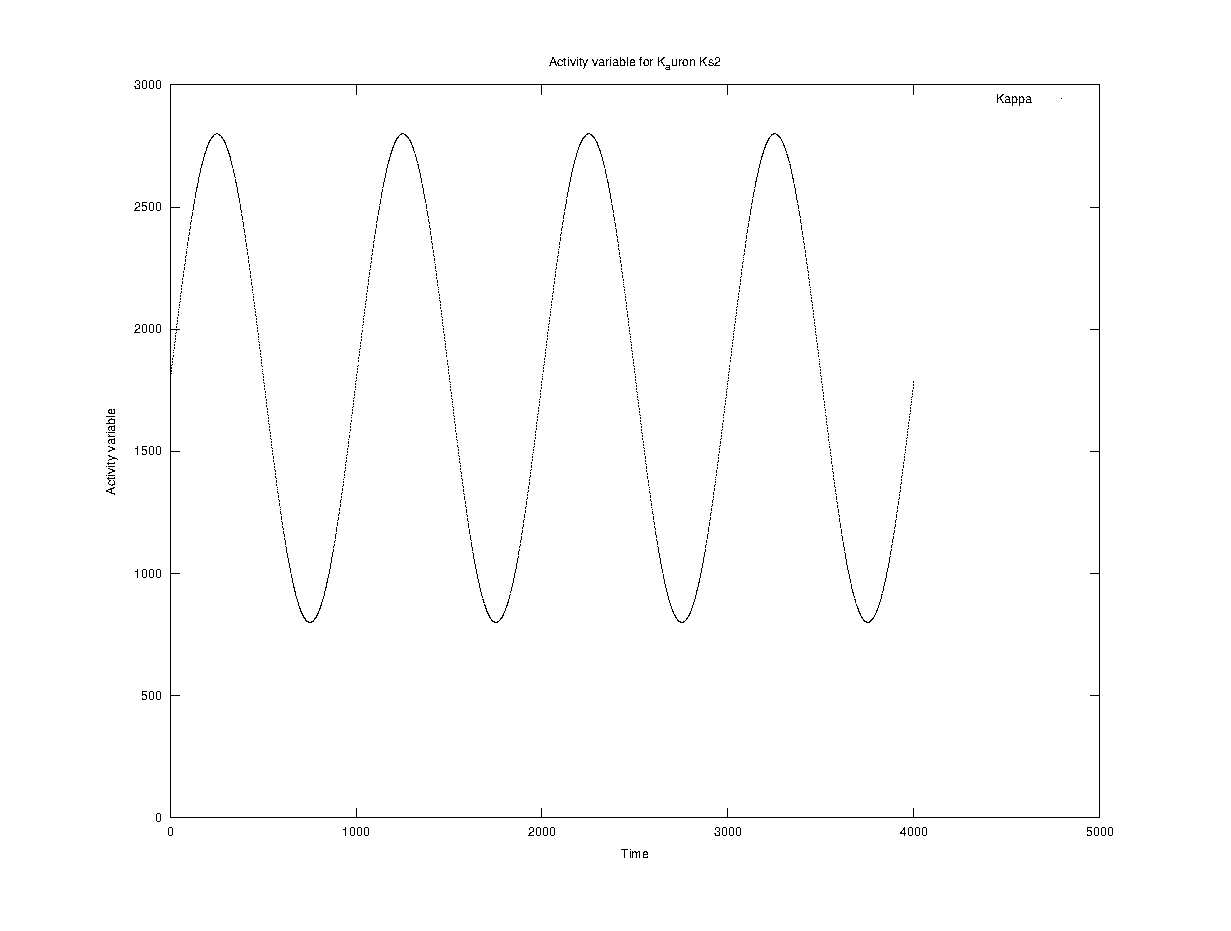
\includegraphics[width=0.5\textwidth]{./synapticTransmissionPlots/eps_auronKs2-kappa.eps} 		} 
   	\subfloat[Synaptic transmission]{\label{figSynTransmission:edge-b} 		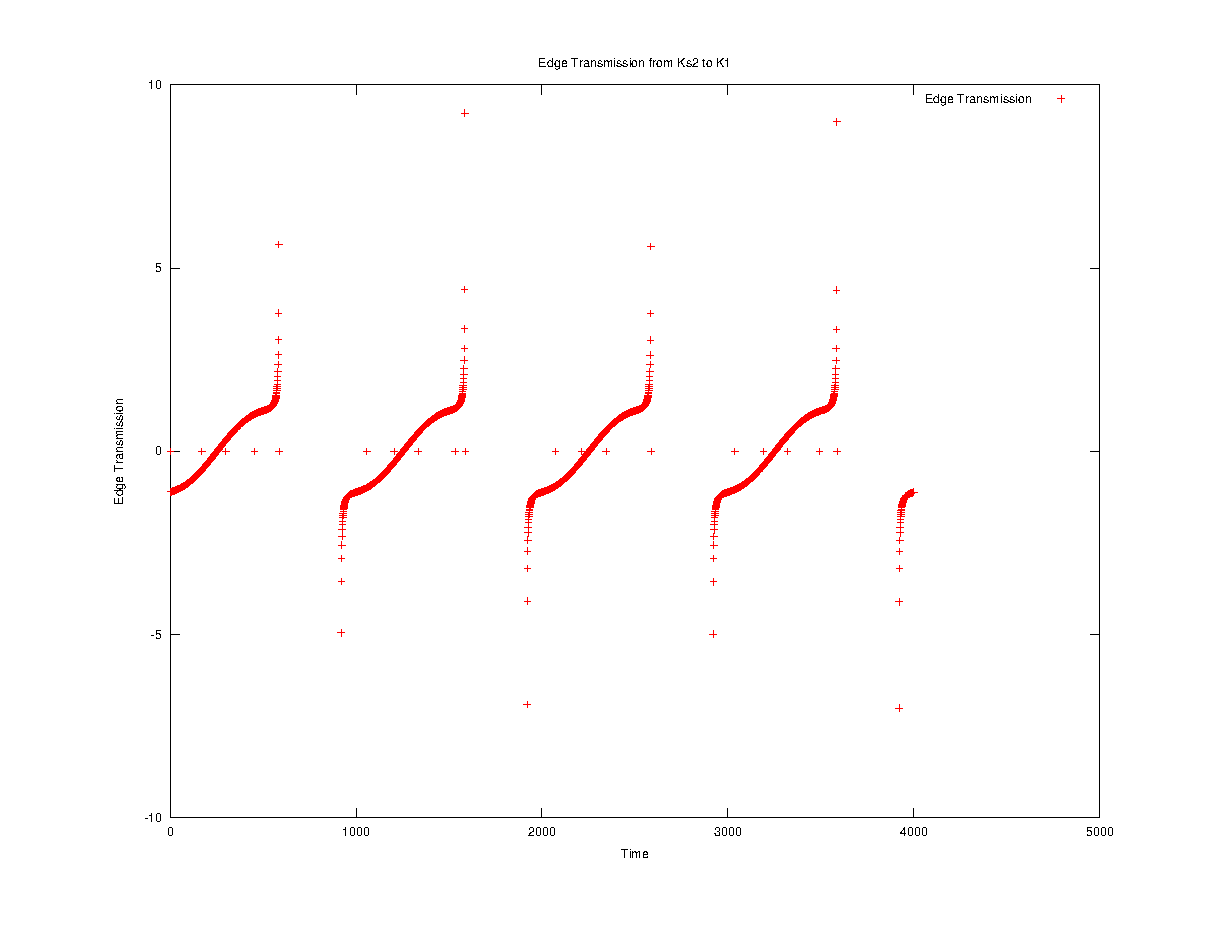
\includegraphics[width=0.5\textwidth]{./synapticTransmissionPlots/eps_transmission_Ks2->K1.eps} 	}
	%\caption{Demonstration of the value function for changing kappa}
	\label{figSynTransmission}
	\caption{The presynapsic activity variable kappa ( \ref{figSynTransmission:edge-a}  ) and the following synaptic transmission ( \ref{figSynTransmission:edge-b} ). 
			Notice the nonlinearity of the synaptic transmission when $\kappa_j \leq \tau$.}
\end{figure}


			When the presynaptic activity variable, $\kappa_j$ varies as a sin( t ) and is at all times above firing threshold, the synaptic transmission will wary as its derived, the cosine.
			%LEGG VED PLOT for [kappa alltid over terskel] også?
			If the presynaptic activity variable as times is equal or below the firing threshold, the plot becomes more interresting.
			Figure \ref{figSynTransmission} shows the presynaptic activity variable, $\kappa_j$ and the following transmission in the synapse. 
			The plots are made from the octave log files following one run of the implementation.

			When $\kappa_j$ approaches the threshold, the presynaptic period goes toward infinity. This causes a synaptic transmission $\kappa_{ij}$ of size zero.
			Since the edge transmission in the implementation is the derived of $\kappa_{ij}$, we get the nonlinearity when $\kappa$ goes below the firing threshold of the presynaptic neuron.
			In the empty interval in the synaptic transmission curve it can be seen that $\kappa_j$ is below the $\tau$, and we do not need to have synaptic transmission.
			% Skrive at dette er ordna med ei if-setning?


		%\subsection{Skrive om implementasjon av dette}
		%\subsection{Skrive om effekter ved denne metoden}
		%	\begin{itemize}
		%		\item At når $\kappa$ nermer seg $\tau$, vil perioden gå mot uendelig veldig raskt. For diskret system vil dette oppfattes som en ulinearitet 
		%		(peride går fra normal verdi til veldig høg verdi -> overføring går "plutselig" til 0). Dette fører til en høg derivert som sørger for at $W_{ij}=0$. Vis transmission plot.
		%		\item at når vi velger å integrere opp den deriverte (overføring) for å finne state, vil vi får 'integral--error' for $\kappa_{post}$.
		%		Dette fører til neste avsnitt: "rekalkulering av Kappa".
		%	\end{itemize}


		\subsection{Relcalculating $\kappa$}
		\label{ssecRecalcKappa}
		Because synaptic transmission is implemented as the derived of the $\kappa_{ij}$, and the postsynaptic activity variable $\kappa_i$ as the integral of this kind of synaptic transmission
		, we have to consider the integral error of $\kappa_i$. 
		Every small error in the calculated $\kappa_i$ will for ever be a part of the result, and we can get potential large errors after a relatively short time.

		For this reason it is important to recalculate $\kappa_i$ periodically.
		The period of recalculating $\kappa$ should find the right balance between recalculating to often, and use to much effort on recalculating $\kappa$, and not recalculating often enough and get integral errors of unacceptable size.

		To best achieve this, the period between recalculating $\kappa$ is dynamic as a function of the error at the last recalcualation. 
		This function should have some kind of maximum when the error is wery small, and a minimum period as the error grows wery large. 

		I have devised an altered sigma function suitable for this purpose.
		\begin{equation}
			\label{eqSigmaFunk}
			p(F) = (c_1+c_2) - \frac{c_2}{1+e^{-(c_4*F-c_3)}}
		\end{equation}


		\begin{figure}[b!htp]
			\label{figSigmaFunk}
			\begin{center}
				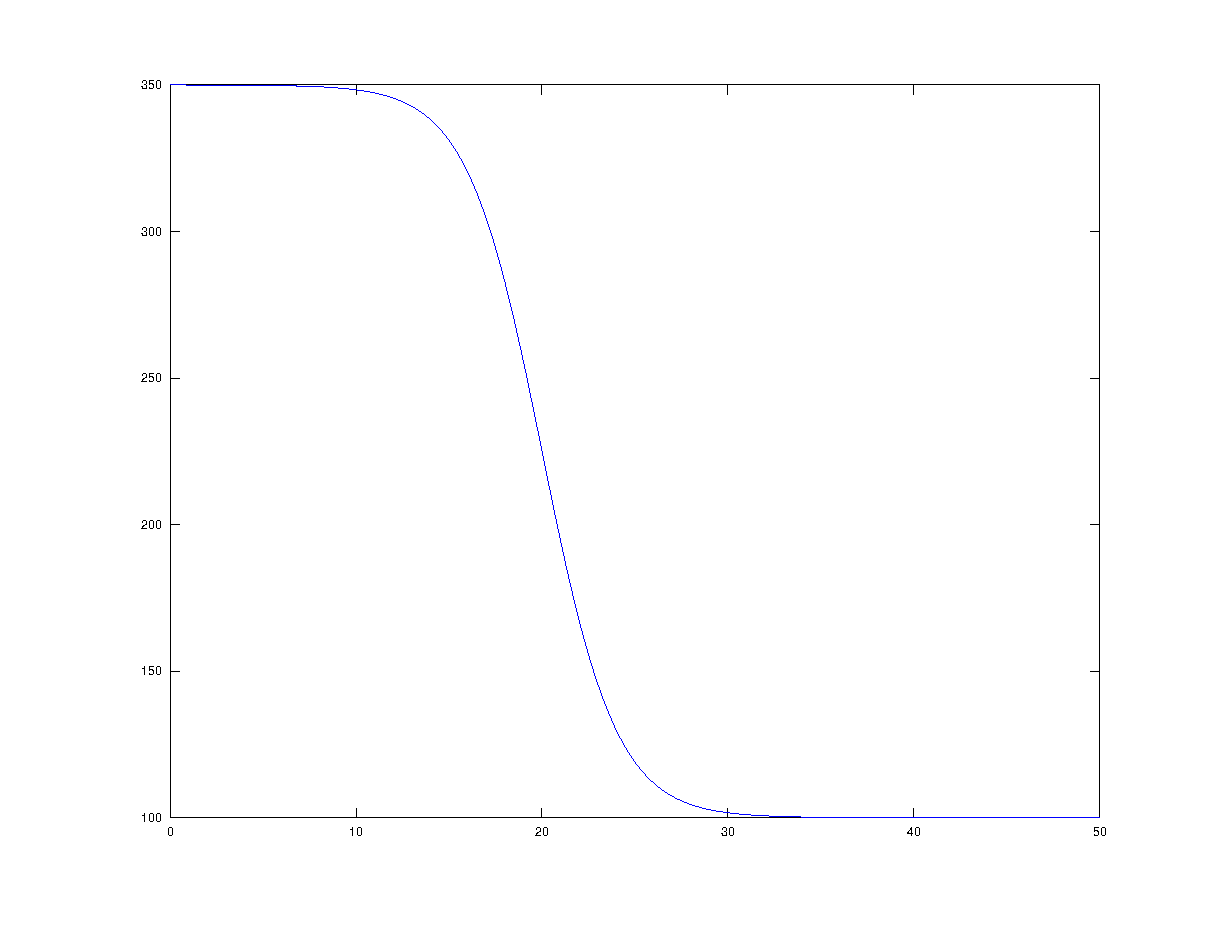
\includegraphics[width=0.95\textwidth]{sigmaPlot.eps}
				%\caption{Demonstration of the value function for changing kappa}
			\end{center}
			\caption{Plot of the altered sigma function (eq. \ref{eqSigmaFunk}), with \mbox{$c_1$ = 100}, \mbox{$c_2$ = 250}, \mbox{$c_3$ = 10} and \mbox{$c_4$ = 0.5} }
		\end{figure}
	
		We can se that \eqref{eqSigmaFunk} has the maximum value of $c_1+c_2$, 350 in figure \ref{figSigmaFunk}. $c_2$ has the value of 250, witch gives the min. value as 100.
		The altered sigma function \eqref{eqSigmaFunk} is used when the period between recalculation of $\kappa$ is calculated. 
		The maximum value, in this context, gives the maximum period before the new recalculation is done. This happens when the error is wery small (se fig \ref{figSigmaFunk}).

		One other thing that is worth noting is the variables $c_3$ and $c_4$ giving the shape of the curve. $c_4$ gives the lenght of the curve, that is how steep it is.
		
		After some analysis, I desided to use the values used in fig. \ref{figSigmaFunk}.
		This gives a function that gives maximum period between recalculation of $\kappa$ when the error is below about 10. 
		It has a relatively steep decent between an error of 10 and 30. The minimum period is set to 100 time steps and the maximum to 350 time iterations.

		The minimum time between recalculation of $\kappa$ will cause the simulation not to use to much resouces.
		The maximum value of this function is limited because the error will have a stocastic nature, and one could e.g. end up with zero error if one get equal positive and negative errors.
		This could give a very large period before the next recalculation of $\kappa$.

		For this reason, the calculation of the period between recalculation of $\kappa$ is also implemented as a FIR--filter with a moving average over the last three values.
		The first time $\kappa$ is calculated, it is calculated with the recalculate function, giving the filter a small initial period, based on the initial level of input.
		If the initial $\kappa$ is large, the first error will be large and the recalculation period will start out as a small period given by the level of input to the node.

		\subsection{Implementation of recalculation of $\kappa$}
		The execution of the planned recalculation of $\kappa$ is done in the same way as the execution of the planned action potential for the $\kappa$ auron.
		In the next section I will use some time on evaluating different methods for executing planned events at the planned time.
		The choice of method for this implementation is described in section \ref{ssChoiceOfTimeEstimationForThisImplementation}.
		
		For recalculation of $\kappa$ with the chosen method, we need a separate object whose doTask() function will call the K\_aurons recalculateKappa() function.
		To achieve this, each K\_auron has its own object of the class recalcKappaClass().

		recalcKappaClass::doTask() then will call the associated K\_aurons recalculateKappa() function, in addition to planning the time of the next recalculation according to the considerations in section \ref{ssecRecalcKappa}.
		

% HER EHER HER er eg.

		%Siden kappa bare regnes ut som integralet av den deriverte, vil det være behov for rekalkulering av Kappa, i ny og ne. Dette bør ikkje skje for ofte, heller ikkje for sjeldent.
		%Difor: lage en adaptiv utførelse av dette. Dette sjekker avviket mellom den rekalkulerte verdien og den gjeldende verdien, ved rekalkulering. 
		%
		%Dette avviket sjekkes opp i mot en predefinert ønska verdi, og differansen er med på å bestemme om periode til neste rekalkulering skal auke eller minke (auker/minker som en funksjon av avvik-avviket). 
		%
		%Dette avviket er m.a.o. med på å bestemme tid til neste rekalkulering av Kappa.
		%Auken/minken bør ha en maksverdi.




	\section{Estimation of firing time}
	For KANN, synaptic transmission can be defined as transmission of change in the postsynaptic node's input level.
	The input of a node, in terms of $\kappa$, is propotional to the synaptic weight and inversly propotional with the presynaptic inter--spike period.

	When the presynaptic node changes its activation level, and its period increases or decreases, the level of synaptic transmission will be altered accordingly. 
	Because of the number of synapses per axon/ dendrite, it is most efficient to perform as many of the calucations as possible in the presynaptic auron.
	For this reason, the most efficient way of calucating the postsynaptic dendrite's activation level is to let the synapse transmit the derived of the signal (change).
	%TODO Har skrevet dette tidligare. (to subsections før). Skriv om, og referer/underbygg denne måten.

	If the transmitted varible is the derived of the signal the postsynaptic dendrite can easily calculate the changed postsynaptic $\kappa_i$, as sen in section \ref{ssecSynInputToANode}.
	% XXX SAGT FØR: If we define $\kappa_{ij}$ as the contribution on $\kappa_i$ from the synapse between node $j$ and node $i$ , $\kappa_i$ can be calculated as
	%\begin{equation}
	%	\kappa_{i} = \sum_j{\kappa_{ij}}
	%\end{equation}
	
	If every $\kappa_{ij}$ but one, $\kappa_{ix}$, is kept constant, it can be shown that $\Delta \kappa_i$ is equal to $\Delta \kappa_{ix}$.
	Following that $\kappa$ is calculated as a superposition of all the input synapses contribution, these equations can be extended to change of transmission of multiple synapses.
	This gives us the equation for the change of postsynaptic activation level following synaptic transmission at synapse from node $x$ to node $i$.

	\begin{equation}
		\kappa_{ij, new} = \kappa_{ij, old} + \Delta \kappa_{ij}
	\end{equation}

	Instead of calculating all of this at every synapse, or for every synapse at the postsynaptic dendrite, it is better to calculate as much as possible presynapticlly.
	This gives one calulation every time a node fires an action potential, instead of one for every output synapse.

	%XXX XXX XXX Trur eg skrive  resten i subsubsection: implementation:KANN -> pEstimatedTaskTime -> execution of elements
	
	% TODO SKRIV litt om dette her, og lag eit frampeik til etter pEstimatedTaskTime, der eg skal skrive meir om dette.
	%Transmission of the derived solves many problems concerning efficiency, but it also introduces integral error for the postsynaptic $\kappa_i$
	%This problem can be solved, and we will come out JAJAJ. Skriv anna gang-- TODO


	%Etterkvart: skriv om integral-errors og fiksing av dette ved å bruke pEstimatedTaskTime (regelmessig fiksing, som er adaptiv med basis i feilen på postsyn signal (høg feil=>oftere regelmessighet på resumming av kappa)).


	When the firing time is estimated, it is fundamental that we have a mechanism for executing these elements at the right time. 
	In the following sections i propose two different solutions for this. 
	In section \ref{ssChoiceOfTimeEstimationForThisImplementation} the choice for this implementation will be presented, and different pros and cons with each method will be discussed.



	
	\subsection{pEstimatedTaskTime}
	$\kappa$ANN is based on calculating the firing time, given the present level of input. 
	Because the input level of an ANN node varies constantly, the calculated firing time is but an estimation of the nodes firing time. 
	The estimation of the nodes firing time changes as the input level does.
	%The estimated firing time for a node changes as the input level does.
	
	The std::list pEstimatedTaskTime is basically an array of dynamic size consisting of std::list--elements,
	where the outer list is an array of future time iterations and the inner lists are arrays of tasks estimated for the respective future time iterations.
	%The inner list is an array of tasks, the outer list is an array of future time iterations. 
	%This can be used for planning the time of execution for different tasks.
	%that keeps overview of when the tasks in the inner tasklist is to be executed.

	The outer list could be said to be the time iteration (relative to the present time iteration) when the tasks in the conlaining list are to be performed. 
	When every task in the inner task list is completed, % ELLER "moved to the pWorkTaskQue" 
		the task list is removed from the outer list. 
	In this way it is possible to keep the relative time--task list updated.

	The tasks located in the inner list of the first element of the outer list are the tasks that are to be executed the next time iteration.
%	Tasks that are to be performed the next time iteration is inserted in the first element (inner list) of the outer list.
%	In time\_class::doTask(), the first element of the outer list (the first inner list) is evaluated, and all the taskt are executed. 
	time\_class::doTask() is responsible for tasks being executed at the planned time. 
	Before time\_class::doTask() iterates time (and moves its pointer from the first element to the last element of pWorkTaskQue), all tasks that are planned for next time iteration is moved from pEstimatedTaskTime to pWorkTaskQue.
	The tasks are appended at the back of pWorkTaskQue before the time\_class object pointer is moved to the end of pWorkTaskQue. 
	This will cause the planned tasks to be performed the next time iteration.

%	Before the discrete time is iterated, the first element is removed from the outer pEstimatedTaskTime--list.
%	In this way it is possible to keep an overview of the immediate future with pEstimatedTaskTime.

	If a new element (a new task) is to be inserted somewhere outside the present scope of the pEstimatedTaskTime, the element (std::list) needs to be constructed.
	Because of the mechanisms of pEstimatedTaskTime, not only the element needs to be produced but also all the estimated time iterations between the length of pEstimatedTaskTime and the estimated time of the respective task.

%dette står lenger nede, under "insertion of elements"
%\begin{lstlisting}
%int nDiff = uRelativeTime - pEstimatedTaskTime.size();
%if( nDiff >= 0 ) //Mangler ledd. Legg til rett antall.
%{
%  for(int i=0; i <= nDiff; i++){
%  pEstimatedTaskTime.push_back( new std::list<timeInterface*> );
%  }
%}
%\end{lstlisting}
	
	\subsubsection{Insertion of elements}
	The std::list container is implemented as a doubly linked list\cite{Stroustrup2000KAP16}.
	To find element nr. $n$ we can iterate throught the list $n$ times from the beginning.
% 	To find element nr. $n$ we can either iterated throught the list ($n$ times) from the beginning, or $S-n$ iterations from the end.
%	An alternative approach if we are concerned with efficiancy, is to iterate from the end that is closest to the element (the beginning or the end of the list).
	In doubly linked lists, we can also iterate thourgh the list from the end.
	If we always iterate from the end that is closest to the target element, the number of iterations required will be halved (if the target position is completely random within a fixed--size list).

	If, for example, we have a list that is 10 elements long and want to access element nr. 9, the most efficient way of doing this in a doubly linked list is to start at the end.
	To generalize this, we can say that if the element that needs to be accessed is later than $\frac{[\text{size of list}]}{2}$ the ``search'' will start at the end.

\begin{lstlisting}
if( uRelativeTime_arg < (pEstimatedTaskTime.size())/2 ){
  // Seach from the last element.
}else{
  // Seach from the first element.
}
\end{lstlisting}

	%If, however, the estimated task time is outside the scope of pEstimatedTaskTime, new elements will have to be inserted.
	Insertion of tasks outside the immediate length of pEstimatedTaskTime requires some attention.
	When an event is planned for some time iteration outside the scope of pEstimatedTaskTime, the scope of pEstimatedTaskTime will have to be increased.
	Because the pEstimatedTaskTime works as a FIFO--que, where the first element % (containing a list of all the planned tasks for the future time iteration)  (se section \ref{ssecEvaluationOfpEstimatedTaskTimeELEMENTS})
		is popped in time\_class::doTask(), it is important to insert every element between the present scope of pEstimatedTaskTime and the new planned task time.
	This is done by
\begin{lstlisting}
int nDiff = uTimeToTask-pEstimatedTaskTime.size();
if( nDiff >= 0){
  for(int i=0; i<=nDiff; i++)
    pEstimatedTaskTime.push_back( new std::list<timeInterface*> );
}
\end{lstlisting}
%This algorithm enshures that pEstimatedTaskTime is correct in terms of time planning.
The expression in the for loop is the reason for having the outer elements of pEstimatedTaskTime defined as std::list$<$timeInterface*$>$ pointers.
In the above algorithm, new std::lists are created in the free store. This creates elements for pEstimatedTaskTime that will exist after the return from the function where the elements are constructed.
%When the free store is used, it is important to deallocate the memory after the element is used. %skriv bedre, denne setininga
To avoid memory exhaustion, it is important to deallocate the memory allocated in the free store when the variable no longer will be used. This is done when the inner lists are evaluated in \emph{time\_class::doTask()}.
For more about the execution of pEstimatedTaskTime tasks, se section \ref{ssecEvaluationOfpEstimatedTaskTimeELEMENTS}.
%TODO Skrim om deallocating memory i ssecEvaluationOfpEstimatedTaskTimeELEMENTS   asd123


	%TODO Koden for denne insertion--funksjonen skal være med i appendix!
	% 			- og skal refereres til fra [her]



%
% 	Skriv om at funk får inn relativ tidsflytt som argument. For å finne relativ tidsflytt trenger eg å lagre gammelTidsPkt i timeInterface-objekt.
% 	Skriv om iterator opplegg. Iterator-returnerende funksjon som søker seg fram til rett ytre-liste (fremtidig tidsiterasjon..)

	\subsubsection{Moving tasks in pEstimatedTaskTime}
	When the planned task time for a timeInterface object is changed, the pointer to the object have to be moved in the pEstimatedTaskTime list.
	
	%In the standard library containers, pointers to elements are called iterators. An iterator 

% TODO TODO TODO TODO TODO TODO TODO TODO TODO TODO TODO TODO TODO TODO TODO TODO
% TODO TODO TODO TODO TODO TODO TODO TODO TODO TODO TODO TODO TODO TODO TODO TOD
% TODO TODO TODO TODO TODO TODO TODO TODO TODO TODO TODO TODO TODO TODO TODO TO
% TODO TODO TODO TODO TODO TODO TODO TODO TODO TODO TODO TODO TODO TODO TODO T
	%TODO lagre heller iteratoren i timeInterface objektet. Tar langt mindre tid. Trur det at iteratoren blir invalidated bare gjelder for vector..
	XXX KORLEIS skal eg gjøre dette? No lagrer eg ulTid i objektet. Kanskje eg heller skal lagre list<list*>::iterator ? Funker dette bedre?
	\emph{Det er bare for vector at iteratoren blir ivalidated når størrelsen på container endre!}

	%Uavhengig av korleis eg finner element, kan eg skrive om flytting av element:
	When the estimated task time is altered, one can assume that the new position will be located not far from the old position, compared to the size of the whole pEstimatedTaskTime list.
	In this case, the most efficient way of finding the new position is to iterate $x$ positions from the old estimated time iteration in pEstimatedTaskTime, instead of finding the position from one of the ends of pEstimatedTaskTime.
	The relative moval of the task can be desided by taking the difference between the new estimate and the old estimate of the task time, $x$, and move the object pointer $x$ iterations along pEstimatedTaskTime. 
	$x$ may be positive or regative.
	
%	\subsubsection{Flytting av element}
%	Implementer først, så skriv om flytting av element som resultat av ny $\kappa$.
%	Element vil ikkje flyttes langt, så beste vil være å flytte elementet fra [no-posisjon].
%	Dette kan lett gjøres i ei `doubly linked list'.
%
%	(planen no er å flytte den ved å ta inn no-iterator-plass (som er lagra i K\_auron) og kor langt den skal flyttes. 
%	Dette gjøres best ved å overlagre funksjonen for når den får argument (iter, timeInterface, tidsFlytt). 
%	Bør returnere iterator, for at auronet skal ha muligheten til å lagre også ny iterator i pEstimatedTaskTime).




	\subsubsection{Evalutation of pEstimatedTaskTime elements}
	%\subsubsection{execution of element tasks}
	\label{ssecEvaluationOfpEstimatedTaskTimeELEMENTS}

	%pEstimatedTaskTime: where all planned tasks for future time iteration lies,
	%pWorkTaskQue: where the tasks for the immediate future lies.
	When the time iteration for the planned events in pEstimatedTaskTime arrives, the tasks in the pEstimatedTaskTime element need execution.

	This can be done by executing the tasks in a separate function, e.g. time\_class::doTask(), that is called at an ideal time for evaluating pEstimatedTaskTime elements.
	%time\_class::doTask() is ideal for executing the tasks. 
	To be consistent about the execution of tasks, it is better to move the tasks planned for the next time iteration from the next element in pEstimatedTaskTime to the pWorkTaskQue list.
	pWorkTaskQue is the list used to plan the immediate future for the ANN, initially developed for the SANN model that focus more on the immediate state of the system.

	When this is done in time\_class::doTask() before time is iterated and the time\_class time separation object is moved to the end of pWorkTaskQue, the tasks from pEstimatedTaskTime will be executed the next time iteration.
	%When the estimated time for the elements task is at the next time iteration, time\_class::doTask() will insert a pointer to the element into pWorkTaskQue.
	%This will will call the node elements \emph{doTask()} function the next time iteration. 

%	The elements of pEstimatedTaskTime is created in the free store, and needs to be deallocated to avoid memory exhaustion. 
	When a pointer to an element is removed from pEstimatedTaskTime, the elements destructor is not called. 
	%When an element is removed from pEstimatedTaskTime, the value of the dereferenced elements destructor is not called because the element is a pointer. 
	It is therefore important to deallocate the memory used for the object in the free store to avoid memory exhaustion.
	%When the element us used and no longer needs to be stored, 
	At the end of time\_class::doTask() this is done explicitly:
\begin{lstlisting}
delete pEstimatedTaskTime.front();
pEstimatedTaskTime.pop_front();
\end{lstlisting}
	The \emph{delete} operator frees the memory allocated to the task list planned for the next time iteration (the dereferenced pointer)
	and the \emph{pop\_front{}} operator removes the now empty pointer in the first element of \emph{pEstimatedTaskTime}.


	

% TODO Skrive eksempel med "the action potential cascade? :
	%I will in the remainder of this section focus on the action potential cascade. 
	%When the firing time of the auron is estimated, a pointer to the auron node element is inserted into pEstimatedTaskTime. 
	%When the time comes for the auron to fire an action potential, the auron pointer is interted into pWorkTaskQue, and the \emph{K\_auron::doTask()} will be executed at the estimated time iteration, inducing the action potential cascade.

	%For K\_aurons, the \emph{doTask()} will first calculate the aurons inverse period (``instantaneous frequency''). 
	%The result is variable \emph{K\_auron::uLastCalculatedPeriod} is made to save this value for later use.
	
	%The new period is calculated, using equation \eqref{eqPeriodeligningForKonstIntraPeriodKAPPA}, giving the level of transmission at the nodes output synapses.
	
	%skriv litt om at denne ligninga er basert på konst. interspike kappa. Dette har vi ikkje her. Kvifor er det viktig alikevel. 
	% 	- delay i ANN. Vente på første spike kan være uoptimalt, men det vil være proposjonalt med aktiviteten, som kan være bra. osv. Drøft (seinare, nevne det her..)
	% 	- arbeidsbelastning.
	

	%\subsection{Checking a member variable of timeInterface--derived elements}
	\subsection{Checking estimated task time directly from time\_class::doTask()}
	A more direct approach is to check the elements estimated firing time directly from time\_class::doTask(). 
	Every class derived from timeInterface contains a variable called ulEstimatedTaskTime where the elements estimated task time is written every time this is updated.
	If we check ulEstimatedTaskTime every time iteration, and number is the same as the next time iteration's index (ulTidsiterasjoner), time\_class::doTask() is responsible to insert its pointer into pWorkTaskQue.
	This will cause the element to do its task on the planned time iteration.
	%If lEstimatedTaskTime is the same as the next time iterations ulTidsiterasjoner, we can insert a pointer to the element into pWorkTaskQue, causing it to do its task next time iteration.

	When $\kappa$ is updated, and K\_auron::doCalculation() updates the aurons estimated firing time, it also updates the K\_auron::lEstimatedTaskTime.
	If $\kappa$ is less than the firing threshold, the K\_aurons lEstimatedTaskTime is set to 0. 

	\subsubsection{Execution of elements}
	time\_class::doTask() runs through the list K\_auron::allKappaAurons to see if any elements have an estimated firing time the next iteration.
	When it finds an element scheduled for the next iteration, the pointer to the element is imnserted into pWorkTaskQue.


	\subsection{Choice for this implementation}
	\ref{ssChoiceOfTimeEstimationForThisImplementation}
	% XXX TODO BEGRUNN GODT KVIFOR EG HAR SKREVET SÅ MYKJE OM pEstimatedTaskTime! Det holder ikkje at eg har gjordt det.
	% 	Skriv at det er godt mulig dette er den mest effektive algoritmen når antall noder auker kraftig!
	% 	Skriv at i såfall må en maks-lengde på lista lages.
	The two methods for execution of tasks at the planned time both have flaws and cons.
	
	pEstimatedTaskTime krever at alle flyttinger av element er riktig. Dersom det er mykje endring av kappa er dette dårlig for denne metoden (krever mykje flytting av element i pEstimatedTaskTime).
	Denne lista er derimot heilt uavhengig av antall auron vi simulerer. For store ANN vil nok denne pEstimatedTaskTime-varianten være best.

	Dersom vi har endring av kappa heile tida, kan metode 2 (den direkte metoden) være best.
	Da koster det ikkje noke å endre fyringsestimatet, men man har en konstant 'cost' ved iterasjon av tid. (BEMERK AT DENNE ER const SEINARE)
	Denne 'cost' er avhengig av antall K\_auron (da den må iterere gjennom alle element [med K>T?]). Denne 'cost' er constant for eit gitt antall auron.

	Det er to grunner til at eg har valt den siste metoden: 1) mine ANN vil være små med mykje endring av kappa. Dette gjør at det er heilt forsvarlig å velge metode nr. 1.
	Den andre grunnen til at eg velger metode nr.1 er at denne har konstant timedelay, noko som er bra..

	jeje... Osv.

	For this implementation, both methods were implemented and tested. 












\subsection{When do $\kappa$ propagate?}
Stavdal meiner at det er tull å propagere heile tida (kvar gang K oppdateres i presyn). 
Eg har laga plot for å sei imot dette: når kappa venter med å propagere til første fyring får man eit tidsdelay for depol til KN tilsvarende tida det tar til første fyring. (dette er veldig tydlig ved sprang i presyn K).

Når Kappa propagerer kvar gang presyn endres, fjærnes dette problemet. Propagerer som det er gjordt før, med at axon legges til i pWorkTaskQue. Alle postsyn. noder får dermed input tidligst neste iterasjon.

Dette har med synapstisk transmissjon å gjøre, og eg må gjøre dette ferdig før eg skrive meir om dette..

NEI faen! no er feilen der igjen. Sjekka kode, og fann at den propagerete, men bare om K>T, så det over er TULL.






%	\subsection{Anna fra tidligare:}
%	-- kanskje skrive om vanskene med log() ? Returnerer samme som argumentet, difor må vi typekonvertere til (float) eller (double) før man tar log() av det. Dette skapte hodebry, siden eg bare fekk resultatet 0.
% 		Ganga med FAKTOR, og fekk 0. Når eg typekonverterte argumenta til log() om til float gjekk fekk eg bra output..

%	Skriv også om at istedenfor å skrive $t_{estimert} = - \frac{1}{\alpha} \ln(\frac{\kappa-\tau}{\kappa-v_0})$ kan eg skrive $t_{estimert} = \frac{1}{\alpha} \ln(\frac{\kappa-v_0}{\kappa-\tau})$
%	(ferre operasjoner, meir effektivt!).

%	\subsection{simulering vha. ligning \eqref{eqVerdiligninga} fra section \ref{secMatematiskModelleringAvBioNeuron}}
%	\subsection{Osv.}












%antagligvis her, men veit ikkje heilt. Iterators. Brukes mykje, så bør forklares (spess for en C patriot)
%\subsection{Skriv om iterators, en plass}
%Dette er veldig viktig for produktet, så bør skrives om.
%
%Iterators er en høgare form for peiker. 
%I standard library er mange basisfunksjoner implementert, og små operatorer (som lenka liste iterering) er lett å implementere.
%Mange små funksjoner som er lett å implementere får alle en liten sannsynlighet for feil. Når det er mange av desse får man mange potensielle feil som er vanskelig å finne.
%
%I standard library er blandt anna en del "containers", som list. Dette er ei ``doubly linked list''.
%Man har også såkalla ``iterators'', som er en peiker til element i slike containers.
%Desse har blandt anna implementert iterator operatoren \emph{++}. Denne er garantert feilfri, og bør brukes fremfor å imlementere slikt selv (seier stroustrup)[referere!].
%
%Skriv at i tillegg til at man kan gå ut  fra at de er feilfri, så er de også godt optimalisert, og vil ofte gi en meir effektiv implementsjon.
%
%Iteratoren har veldig masse til felles med en peiker, bare med lettere, feilfri, meir optimalisert utførelse.


%\subsubsection{Ikkje mulig å lagre iteratoren}
%ELLER ER DET MULIG? (Kan være det under bare gjelder for vector!)
%
%Iteratore blir ugyldige, og gir udefinert oppførsel dersom lista blir rezised i mellom iteratoren blir laget og brukt. 
%Initiellt var tanken at K\_auron (og kanskje andre timeInterface som bruker pEstimatedTaskTime) skulle også inneholde en iterator (peiker) til rett element i lista.
%Siden iteratore blir ugyldig når listas lengde endres %stroustrup s. 550, nede. Understreka.
%	så går ikkje dette.
%
%Dette er grunnen til at kvar gang eit element skal flyttes, må det søkes opp på nytt (forrige plass kan inneholde eit nytt element, eller være forbi slutten av lista..)
%
%Siden vi ikkje bør anta kor den er, bør lista itereres gjennom på nytt. 
%En antagelse som er trygg er at elementet ikkje har flyttet seg veldig langt, når estimatet oppdateres.
%Dette gjør at det antagelig ligger i samme halvdel av lista, og det kan være lurt å begynne søket fra den siden som er nærmast ny plassering. %type før eller etter size() / 2 , før => start søk fra starten ...
%
%For å effektivisere, lages to funksjoner: en som legger til element, og en som flytter det. 
%Ved fyring av K\_auron fjærnes elementet, men skal også legges til på tidspkt. [no]+[estimert periode].
%Løsninga mi blir: i funksjonen som fjærner elementet, vil også nytt element legges til om element->periode. Dette er en rein insertion.
%
%For flytting av element må lista itereres gjennom, og kvar iterasjon må lista--elementet gjennomsøkes etter gjeldende element. 
%Dette er meir tidkrevende, og er grunnen til at eg skiller mellom de to operasjonene: insertion og moving of an element.
%
%Les stroustrup s. 550 for meir, når dette skal skrives om!







